\documentclass{article}
\usepackage[utf8]{inputenc}
\usepackage{amsmath,amssymb}
\usepackage{tikz}
\usepackage{pgfplots}
\usepackage{hyperref}
\usepackage{xcolor}

% Load additional TikZ libraries
\usetikzlibrary{arrows.meta}
\usetikzlibrary{shapes.geometric}
\usetikzlibrary{decorations.pathmorphing}
\usetikzlibrary{decorations.markings}
\usetikzlibrary{patterns}
\usetikzlibrary{positioning}
\usetikzlibrary{mindmap}
\usetikzlibrary{trees}
\usetikzlibrary{calc}

% PGFPlots settings
\pgfplotsset{compat=1.18}

\title{TikZ and PGFPlots Gallery}
\author{GitHub Actions Demo}
\date{\today}

\begin{document}

\maketitle

\begin{abstract}
  This document showcases various TikZ and PGFPlots examples to demonstrate how they are converted to SVG in the HTML output. The examples range from simple shapes to complex diagrams, charts, and plots.
\end{abstract}

\section{Introduction}

TikZ (TikZ ist kein Zeichenprogramm) is a powerful package for creating graphics in \LaTeX. PGFPlots is built on top of TikZ and provides tools for creating scientific plots. This document demonstrates how these packages can be used to create various types of diagrams and how they are converted to SVG in the HTML output.

\section{Basic Shapes and Paths}

\subsection{Simple Shapes}

\begin{figure}[h]
  \centering
  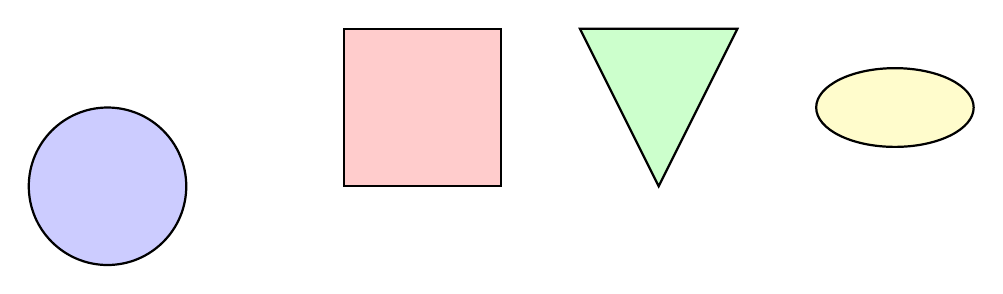
\begin{tikzpicture}
    % Circle
    \draw[thick, fill=blue!20] (0,0) circle (1cm);
    % Rectangle
    \draw[thick, fill=red!20] (3,0) rectangle (5,2);
    % Triangle
    \draw[thick, fill=green!20] (7,0) -- (8,2) -- (6,2) -- cycle;
    % Ellipse
    \draw[thick, fill=yellow!20] (10,1) ellipse (1cm and 0.5cm);
  \end{tikzpicture}
  \caption{Basic shapes in TikZ: circle, rectangle, triangle, and ellipse}
\end{figure}

\subsection{Lines and Arrows}

\begin{figure}[h]
  \centering
  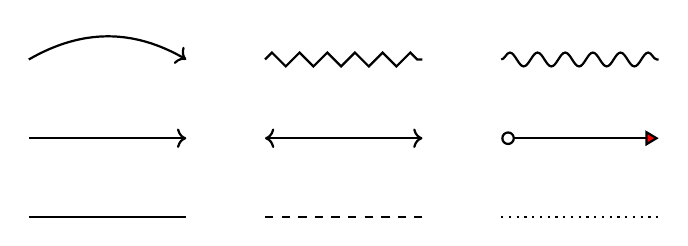
\begin{tikzpicture}
    % Straight line
    \draw[thick] (0,0) -- (2,0);
    % Dashed line
    \draw[thick, dashed] (3,0) -- (5,0);
    % Dotted line
    \draw[thick, dotted] (6,0) -- (8,0);
    % Arrow
    \draw[thick, ->] (0,1) -- (2,1);
    % Double arrow
    \draw[thick, <->] (3,1) -- (5,1);
    % Custom arrow
    \draw[thick, {Circle[open]}-{Triangle[fill=red]}] (6,1) -- (8,1);
    % Curved arrow
    \draw[thick, ->, bend left] (0,2) to (2,2);
    % Zigzag line
    \draw[thick, decorate, decoration={zigzag}] (3,2) -- (5,2);
    % Wave line
    \draw[thick, decorate, decoration={snake}] (6,2) -- (8,2);
  \end{tikzpicture}
  \caption{Various line styles and arrows in TikZ}
\end{figure}

\section{Diagrams and Charts}

\subsection{Flowchart}

\begin{figure}[h]
  \centering
  \begin{tikzpicture}[node distance=2cm, auto]
    % Define styles
    \tikzstyle{decision} = [diamond, draw, fill=blue!20, text width=4.5em, text badly centered, inner sep=0pt]
    \tikzstyle{block} = [rectangle, draw, fill=blue!20, text width=5em, text centered, rounded corners, minimum height=4em]
    \tikzstyle{line} = [draw, -latex']
    
    % Place nodes
    \node [block] (init) {Initialize};
    \node [block, below of=init] (process) {Process};
    \node [decision, below of=process] (decide) {Decision?};
    \node [block, below left of=decide, xshift=-1.5cm] (yes) {Yes};
    \node [block, below right of=decide, xshift=1.5cm] (no) {No};
    \node [block, below of=yes, xshift=1.5cm] (end) {End};
    
    % Connect nodes
    \path [line] (init) -- (process);
    \path [line] (process) -- (decide);
    \path [line] (decide) -- node [near start] {yes} (yes);
    \path [line] (decide) -- node [near start] {no} (no);
    \path [line] (yes) |- (end);
    \path [line] (no) |- (end);
  \end{tikzpicture}
  \caption{A simple flowchart using TikZ}
\end{figure}

\subsection{Mind Map}

\begin{figure}[h]
  \centering
  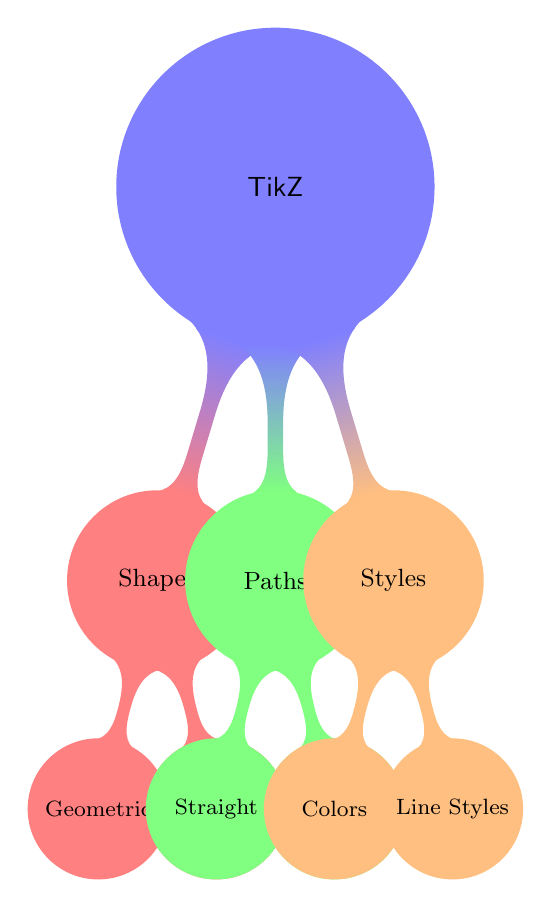
\begin{tikzpicture}[mindmap, concept color=blue!50, font=\sffamily]
    \node[concept] {TikZ}
      child[concept color=red!50] { node[concept] {Shapes}
        child { node[concept] {Geometric} }
        child { node[concept] {Arrows} }
      }
      child[concept color=green!50] { node[concept] {Paths}
        child { node[concept] {Straight} }
        child { node[concept] {Curved} }
      }
      child[concept color=orange!50] { node[concept] {Styles}
        child { node[concept] {Colors} }
        child { node[concept] {Line Styles} }
      };
  \end{tikzpicture}
  \caption{A mind map created with TikZ}
\end{figure}

\subsection{Tree Diagram}

\begin{figure}[h]
  \centering
  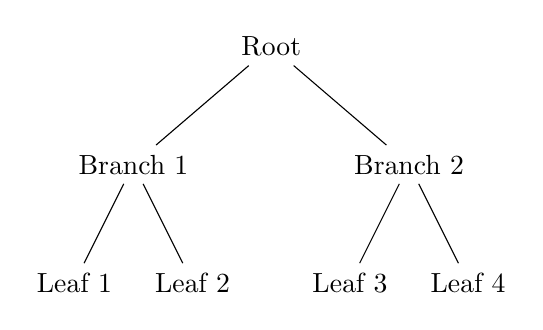
\begin{tikzpicture}[level distance=1.5cm,
    level 1/.style={sibling distance=3.5cm},
    level 2/.style={sibling distance=1.5cm}]
    \node {Root}
      child { node {Branch 1}
        child { node {Leaf 1} }
        child { node {Leaf 2} }
      }
      child { node {Branch 2}
        child { node {Leaf 3} }
        child { node {Leaf 4} }
      };
  \end{tikzpicture}
  \caption{A tree diagram using TikZ}
\end{figure}

\subsection{UML Class Diagram}

\begin{figure}[h]
  \centering
  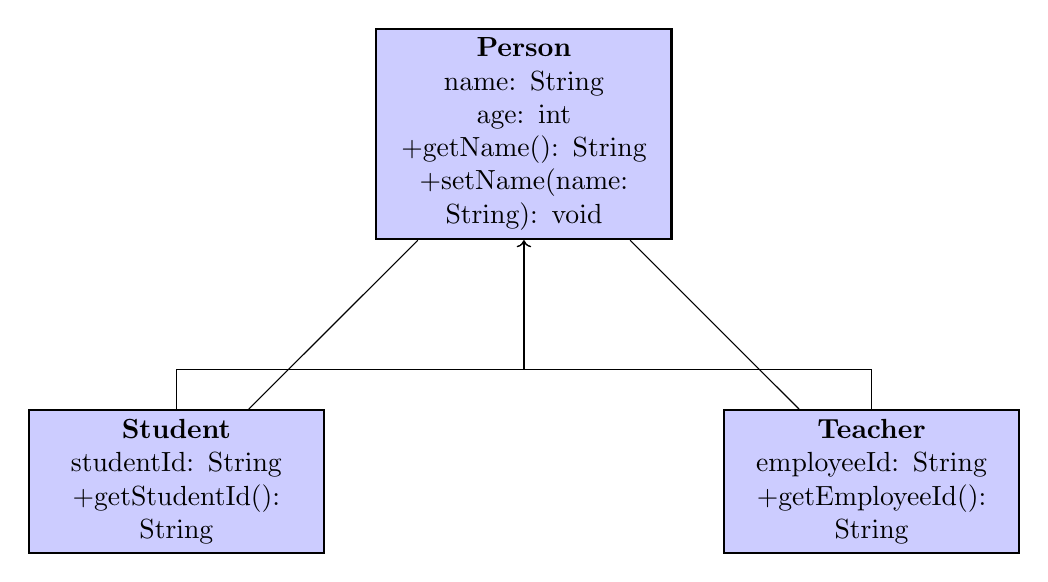
\begin{tikzpicture}[node distance=2cm, auto]
    % Define styles
    \tikzstyle{class} = [rectangle, draw=black, thick, fill=blue!20, text width=10em, text centered, minimum height=2.5em, minimum width=10em]
    \tikzstyle{line} = [draw, -]
    
    % Place nodes
    \node [class] (person) {\textbf{Person}\\name: String\\age: int\\+getName(): String\\+setName(name: String): void};
    
    \node [class, below left of=person, xshift=-3cm, yshift=-3cm] (student) {\textbf{Student}\\studentId: String\\+getStudentId(): String};
    
    \node [class, below right of=person, xshift=3cm, yshift=-3cm] (teacher) {\textbf{Teacher}\\employeeId: String\\+getEmployeeId(): String};
    
    % Connect nodes
    \path [line] (student) -- (person);
    \path [line] (teacher) -- (person);
    
    % Add inheritance arrows
    \draw[->] (student.north) -- ++(0,0.5) -| (person.south);
    \draw[->] (teacher.north) -- ++(0,0.5) -| (person.south);
  \end{tikzpicture}
  \caption{A UML class diagram using TikZ}
\end{figure}

\section{Plots with PGFPlots}

\subsection{2D Function Plots}

\begin{figure}[h]
  \centering
  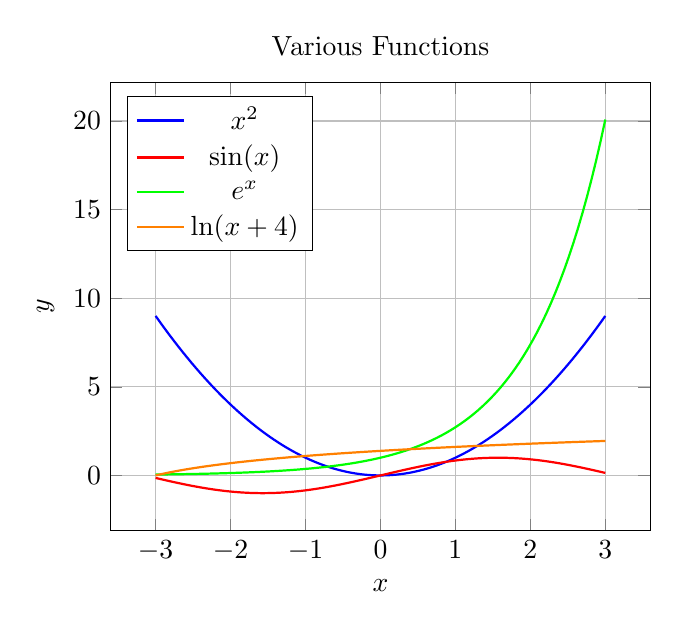
\begin{tikzpicture}
    \begin{axis}[
      xlabel={$x$},
      ylabel={$y$},
      title={Various Functions},
      legend pos=north west,
      grid=both,
      domain=-3:3,
      samples=100
    ]
      \addplot[blue, thick] {x^2};
      \addplot[red, thick] {sin(deg(x))};
      \addplot[green, thick] {exp(x)};
      \addplot[orange, thick] {ln(x+4)};
      \legend{$x^2$, $\sin(x)$, $e^x$, $\ln(x+4)$}
    \end{axis}
  \end{tikzpicture}
  \caption{Various function plots using PGFPlots}
\end{figure}

\subsection{Bar Chart}

\begin{figure}[h]
  \centering
  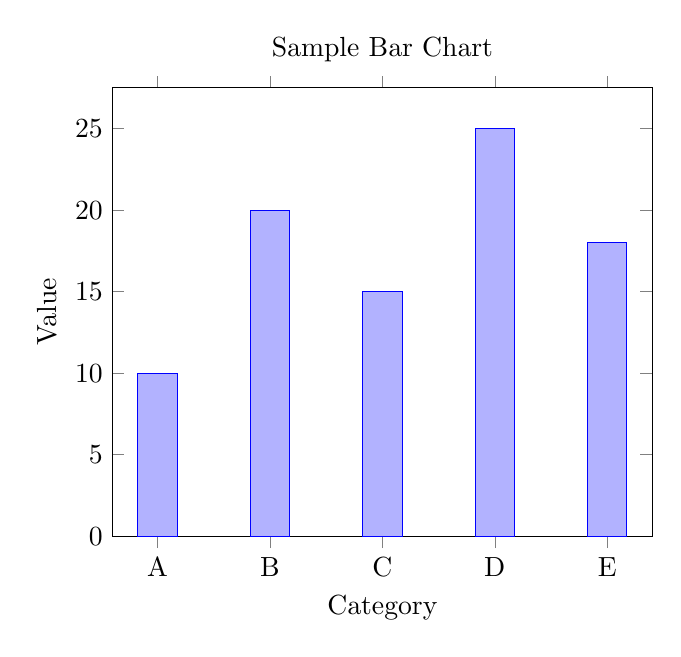
\begin{tikzpicture}
    \begin{axis}[
      xlabel={Category},
      ylabel={Value},
      title={Sample Bar Chart},
      symbolic x coords={A, B, C, D, E},
      xtick=data,
      ybar,
      bar width=0.5cm,
      ymin=0
    ]
      \addplot coordinates {(A, 10) (B, 20) (C, 15) (D, 25) (E, 18)};
    \end{axis}
  \end{tikzpicture}
  \caption{A bar chart using PGFPlots}
\end{figure}

\subsection{Scatter Plot}

\begin{figure}[h]
  \centering
  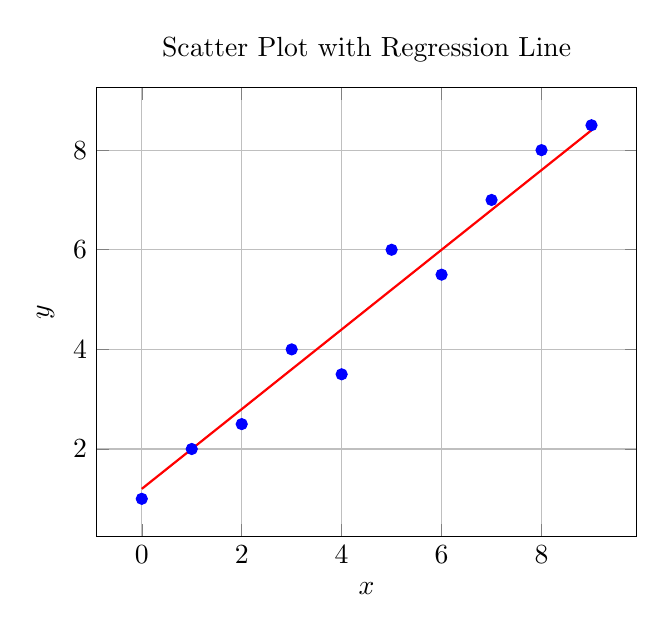
\begin{tikzpicture}
    \begin{axis}[
      xlabel={$x$},
      ylabel={$y$},
      title={Scatter Plot with Regression Line},
      grid=both
    ]
      % Scatter plot
      \addplot[only marks, mark=*, blue] coordinates {
        (0, 1) (1, 2) (2, 2.5) (3, 4) (4, 3.5) (5, 6) (6, 5.5) (7, 7) (8, 8) (9, 8.5)
      };
      % Linear regression line
      \addplot[red, thick, domain=0:9] {0.8*x + 1.2};
    \end{axis}
  \end{tikzpicture}
  \caption{A scatter plot with a regression line using PGFPlots}
\end{figure}

\subsection{3D Surface Plot}

\begin{figure}[h]
  \centering
  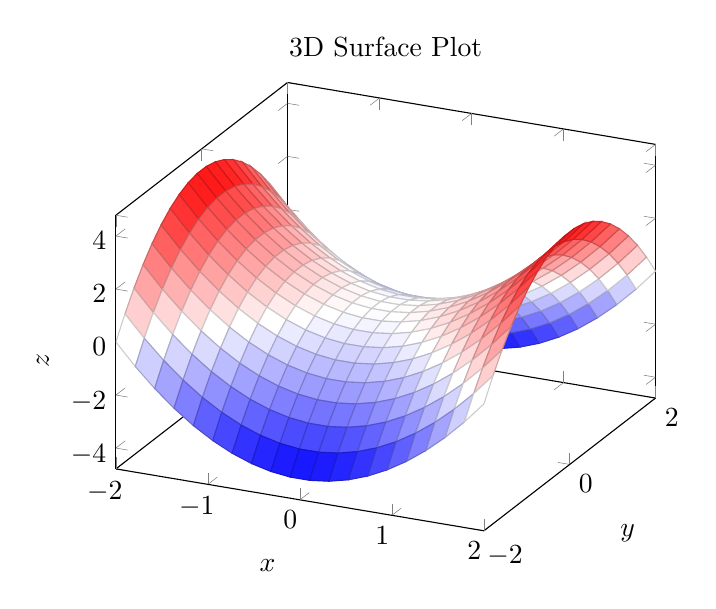
\begin{tikzpicture}
    \begin{axis}[
      xlabel={$x$},
      ylabel={$y$},
      zlabel={$z$},
      title={3D Surface Plot},
      colormap={bluewhitered}{color(0cm)=(blue); color(1cm)=(white); color(2cm)=(red)}
    ]
      \addplot3[
        surf,
        domain=-2:2,
        domain y=-2:2,
        samples=20
      ] {x^2 - y^2};
    \end{axis}
  \end{tikzpicture}
  \caption{A 3D surface plot using PGFPlots}
\end{figure}

\section{Advanced Examples}

\subsection{Circuit Diagram}

\begin{figure}[h]
  \centering
  \begin{tikzpicture}[circuit ee IEC, thick]
    % Define components
    \draw (0,0) to [battery] (0,3) to [resistor] (3,3) to [lamp] (6,3) to [switch] (6,0) to [ground] (6,-1);
    \draw (6,0) -- (0,0);
    
    % Add labels
    \node at (0,1.5) [left] {Battery};
    \node at (3,3) [above] {Resistor};
    \node at (6,3) [above] {Lamp};
    \node at (6,0) [right] {Switch};
  \end{tikzpicture}
  \caption{A simple circuit diagram using TikZ}
\end{figure}

\subsection{Chemical Diagram}

\begin{figure}[h]
  \centering
  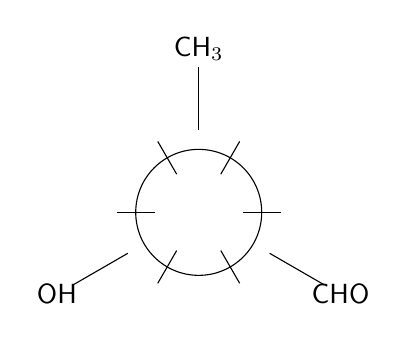
\begin{tikzpicture}[font=\sffamily, scale=0.8]
    % Benzene ring
    \draw (0,0) circle (1cm);
    \foreach \i in {0,60,...,300} {
      \draw (\i:0.7cm) -- (\i:1.3cm);
    }
    
    % Methyl group
    \draw (90:1.3cm) -- (90:2.3cm);
    \node at (90:2.6cm) {CH$_3$};
    
    % Hydroxyl group
    \draw (210:1.3cm) -- (210:2.3cm);
    \node at (210:2.6cm) {OH};
    
    % Aldehyde group
    \draw (330:1.3cm) -- (330:2.3cm);
    \node at (330:2.6cm) {CHO};
  \end{tikzpicture}
  \caption{A chemical structure diagram using TikZ}
\end{figure}

\subsection{Commutative Diagram}

\begin{figure}[h]
  \centering
  \begin{tikzpicture}[scale=1.5]
    \node (A) at (0,2) {$A$};
    \node (B) at (2,2) {$B$};
    \node (C) at (0,0) {$C$};
    \node (D) at (2,0) {$D$};
    
    \draw[->] (A) -- node[above] {$f$} (B);
    \draw[->] (A) -- node[left] {$g$} (C);
    \draw[->] (B) -- node[right] {$h$} (D);
    \draw[->] (C) -- node[below] {$i$} (D);
  \end{tikzpicture}
  \caption{A commutative diagram using TikZ}
\end{figure}

\section{Conclusion}

This document has demonstrated various TikZ and PGFPlots examples that can be converted to SVG in the HTML output. The GitHub Actions workflow handles the conversion process, ensuring that all diagrams are properly rendered in the final HTML document.

The examples shown here range from simple shapes to complex diagrams and plots, showcasing the versatility of TikZ and PGFPlots for creating high-quality graphics in \LaTeX documents.

\end{document}